\documentclass[10pt]{article}
\usepackage[english]{babel}
\usepackage{../../../meta-inf/lib/naproche}
\usepackage{amssymb}
\usepackage{mathtools} % for \coloneq

\usepackage{stex-highlighting}
\providebool{emph} % "\newbool{emph}" does not work...
\setbool{emph}{false}
\colorlet{emphcolor}{violet}
\let\oldemph\emph
\renewcommand\emph[1]{\setbool{emph}{true}\ifbool{forthel}{\textcolor{emphcolor}{\itshape#1}}{\oldemph{#1}}\setbool{emph}{false}}
\renewcommand{\varemph}[1]{\ifbool{emph}{\textcolor{emphcolor}{#1}}{\textcolor{black}{#1}}}

\usepackage[right=6cm,left=3cm,bottom=3cm,marginparwidth=5cm]{geometry}

\usepackage{fancyhdr}
\renewcommand{\sectionmark}[1]{\markboth{#1}{}} 
\def\libarchive{}
\pagestyle{fancy}
\fancyhead[L]{\libarchive}
\fancyhead[C]{\nouppercase\leftmark}  % section title
\fancyhead[R]{\thepage}               % page number
\fancyfoot[C]{}                       % No page number in footer

\usepackage[nobottomtitles]{titlesec}
\titlespacing*{\section}{0pt}{30pt}{0pt}
\titlespacing*{\subsection}{0pt}{30pt}{0pt}
\titlespacing*{\subsubsection}{0pt}{30pt}{0pt}

\documentclass[12pt,oneside]{book}

\usepackage[foundations]{../../lib/tex/naproche}
\usepackage{../../lib/tex/libraries}
\usepackage{graphicx}
\usepackage{float}
\usepackage{caption}
\usepackage{footnote}

\makesavenoteenv{tabular} % Make footnotes work in tabular environments


\title{Foundations of Mathematics}
\author{Marcel Schütz}
\date{2022}

\begin{document}
  \maketitle

  \tableofcontents

  \begin{figure}[H]
    \centering
    \fbox{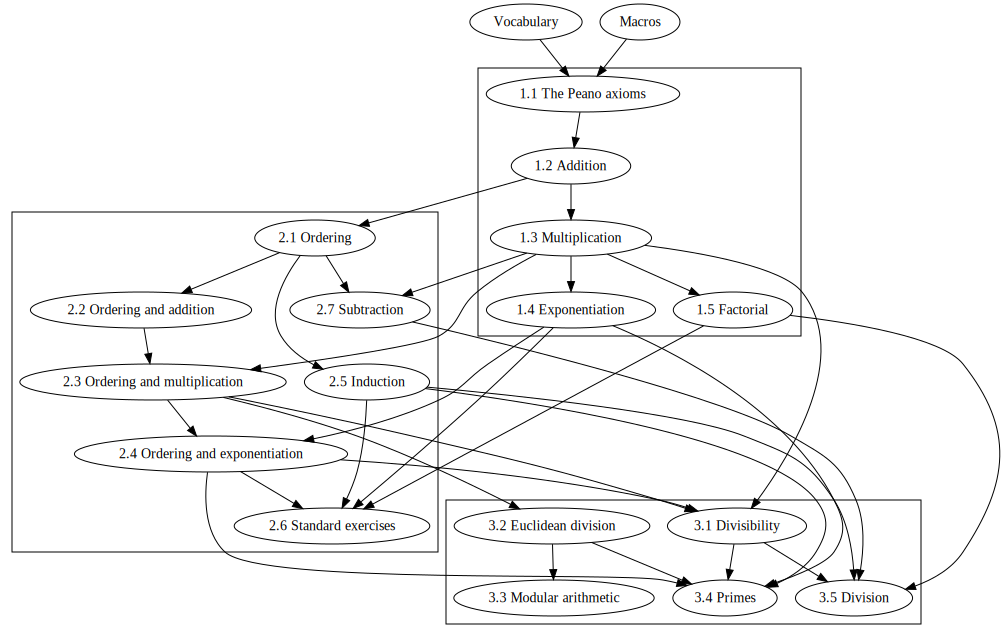
\includegraphics[width=0.9\linewidth]{./dependency-graph/graph.png}}
    \caption*{Interdependencies of the chapters}
  \end{figure}


  \section*{Introduction}

  This is a library providing a foundation of mathematics based on a
  Kelley-Morse like class theory with urelements.
  It introduces common operations on classes like unions or intersections
  (\cref{chapter:classes}) together with detailed proofs of their algebraic
  properties (\cref{chapter:computation-laws-for-classes}), the symmetric
  difference of two classes (\cref{chapter:symmetric-difference}) and the
  notions of ordered pairs and Cartesian products
  (\cref{chapter:pairs-and-products}) as well as proofs of the algebraic
  properties of the latter (\cref{chapter:computation-laws-for-products}).
  Moreover, it provides common operations on maps (\cref{chapter:maps}), various
  properties of images and preimages (\cref{chapter:image-and-preimage}) and the
  notions of injectivity, surjectivity, bijectivity
  (\cref{chapter:injections-surjections-bijections}) and invertibility of maps
  (\cref{chapter:invertible-maps}).
  The library provides an axiom system characterizing sets (\cref{chapter:sets})
  and, furthermore, it covers the notions of binary relations
  (\cref{chapter:binary-relations}), fixed-points of subset preserving maps
  (\cref{chapter:fixed-points}), including and equinumerosity
  (\cref{chapter:equinumerosity}).

  As two famous results it includes the Knaster-Tarski fixed point theorem
  (\cref{FOUNDATIONS_12_8420450166112256}) and the Cantor-Schröder-Bernstein
  theorem (\cref{FOUNDATIONS_13_1913663275401216}).

  \paragraph*{Usage.}
  At the very beginning of each chapter you can find the name of its source
  file, e.g. \path{foundations/sections/01_classes.ftl.tex} for
  \cref{chapter:classes}. This filename can be used to import the chapter via
  \Naproche's \texttt{readtex} instruction to another ForTheL text, e.g.:
  \begin{center}
    \verb`[readtex \path{foundations/sections/01_classes.ftl.tex}]`
  \end{center}

  \paragraph*{Checking times.}
  The checking times for each of the chapters may vary from computer to
  computer, but on mid-range hardware they are likely to be similar to those
  given in table below:

  \begin{center}
    \begin{tabular}{c|c|c}

      & \multicolumn{2}{c}{\textbf{Checking time}}
      \\
      \textbf{Chapter}
      & \textbf{without dependencies}     & \textbf{with dependencies}
      \\ \hline
      \ref{chapter:classes}
      & 00:04 min                         & 00:04 min
      \\
      \ref{chapter:computation-laws-for-classes}
      & 00:12 min                         & 00:16 min
      \\
      \ref{chapter:symmetric-difference}
      & 00:32 min                         & 00:48 min
      \\
      \ref{chapter:pairs-and-products}
      & 00:08 min                         & 00:12 min
      \\
      \ref{chapter:computation-laws-for-products}
      & 01:36 min                         & 01:56 min
      \\
      \ref{chapter:maps}
      & 01:13 min                         & 01:25 min
      \\
      \ref{chapter:image-and-preimage}
      & 01:28 min                         & 02:53 min
      \\
      \ref{chapter:injections-surjections-bijections}
      & 00:38 min                         & 02:03 min
      \\
      \ref{chapter:invertible-maps}
      & 02:20 min                         & 04:23 min
      \\
      \ref{chapter:sets}
      & 02:17 min                         & 06:40 min
      \\
      \ref{chapter:binary-relations}
      & 00:14 min                         & 06:54 min
      \\
      \ref{chapter:fixed-points}
      & 00:33 min                         & 07:13 min
      \\
      \ref{chapter:equinumerosity}
      & 01:48 min                         & 09:01 min
    \end{tabular}
  \end{center}


  \subfile{sections/01_classes.ftl.tex}
  \subfile{sections/02_computation-laws-for-classes.ftl.tex}
  \subfile{sections/03_symmetric-difference.ftl.tex}
  \subfile{sections/04_pairs-and-products.ftl.tex}
  \subfile{sections/05_computation-laws-for-products.ftl.tex}
  \subfile{sections/06_maps.ftl.tex}
  \subfile{sections/07_image-and-preimage.ftl.tex}
  \subfile{sections/08_injections-surjections-bijections.ftl.tex}
  \subfile{sections/09_invertible-maps.ftl.tex}
  \subfile{sections/10_sets.ftl.tex}
  \subfile{sections/11_binary-relations.ftl.tex}
  \subfile{sections/12_fixed-points.ftl.tex}
  \subfile{sections/13_equinumerosity.ftl.tex}
\end{document}

\usepackage{amssymb}

\newcommand{\Nat}{\mathbb{N}}
\newcommand{\Prime}{\mathbb{P}}
\renewcommand{\succ}{\textrm{succ}}
\newcommand{\pred}{\textrm{pred}}
\newcommand{\add}{\textrm{add}}
\newcommand{\mul}{\textrm{mul}}
\renewcommand{\exp}{\textrm{exp}}
\newcommand{\fac}{\textrm{fac}}
\renewcommand{\div}{\mathop{\textrm{div}}}
\renewcommand{\mod}{\mathop{\textrm{mod}}}

\begin{document}
  \begin{imports}
    \begin{forthel}
      %[prove off][check off]
      [readtex \path{libraries/source/foundations/classes.ftl.tex}]
      %[prove on][check on]
    \end{forthel}
  \end{imports}


  \section*{Natural Numbers}

  \subsection*{The Language of Natural Number Arithmetic}

  \begin{forthel}
    \begin{signature}[id=ARITHMETIC_01_3074681254969344,printid]
      A natural number is an object.
    \end{signature}
  \end{forthel}

  \begin{forthel}
    \begin{definition}[id=ARITHMETIC_01_7367148418629632,printid]
      $\Nat$ is the class of natural numbers.
    \end{definition}
  \end{forthel}

  \begin{forthel}
    \begin{signature}[id=ARITHMETIC_01_1567933815848960,printid]
      Let $n, m$ be natural numbers.
      $n + m$ is a natural number.
    \end{signature}

    Let the sum of $n$ and $m$ stand for $n + m$.
  \end{forthel}

  \begin{forthel}
    \begin{signature}[id=ARITHMETIC_01_7633304715001856,printid]
      $0$ is a natural number.
    \end{signature}

    Let zero stand for $0$.
    Let $n$ is nonzero stand for $n \neq 0$.
  \end{forthel}

  \begin{forthel}
    \begin{signature}[id=ARITHMETIC_01_1200254566985232,printid]
      $1$ is a natural number.
    \end{signature}

    Let one stand for $1$.
    Let the direct successor of $n$ stand for $n + 1$.
  \end{forthel}
  
  \begin{forthel}
    \begin{definition}[id=ARITHMETIC_01_4584236572999680,printid]
      $2 = 1 + 1$.
    \end{definition}

    Let two stand for $2$.
  \end{forthel}

  \begin{forthel}
    \begin{definition}[id=ARITHMETIC_01_3836725109456896,printid]
      $3 = 2 + 1$.
    \end{definition}

    Let three stand for $3$.
  \end{forthel}

  \begin{forthel}
    \begin{definition}[id=ARITHMETIC_01_1709884968009728,printid]
      $4 = 3 + 1$.
    \end{definition}

    Let four stand for $4$.
  \end{forthel}

  \begin{forthel}
    \begin{definition}[id=ARITHMETIC_01_6734726333202432,printid]
      $5 = 4 + 1$.
    \end{definition}

    Let five stand for $5$.
  \end{forthel}

  \begin{forthel}
    \begin{definition}[id=ARITHMETIC_01_949139189792768,printid]
      $6 = 5 + 1$.
    \end{definition}

    Let six stand for $6$.
  \end{forthel}

  \begin{forthel}
    \begin{definition}[id=ARITHMETIC_01_7245471749767168,printid]
      $7 = 6 + 1$.
    \end{definition}

    Let seven stand for $7$.
  \end{forthel}

  \begin{forthel}
    \begin{definition}[id=ARITHMETIC_01_5658172888973312,printid]
      $8 = 7 + 1$.
    \end{definition}

    Let eight stand for $8$.
  \end{forthel}

  \begin{forthel}
    \begin{definition}[id=ARITHMETIC_01_7371844250238976,printid]
      $9 = 8 + 1$.
    \end{definition}

    Let nine stand for $9$.
  \end{forthel}


  \subsection*{The Axioms of Natural Number Arithmetic}

  \begin{forthel}
    \begin{axiom}[id=ARITHMETIC_01_3604163883696128,printid]
      Let $n, m$ be natural numbers.
      If $n + 1 = m + 1$ then $n = m$.
    \end{axiom}
  \end{forthel}

  \begin{forthel}
    \begin{axiom}[id=ARITHMETIC_01_4454289938317312,printid]
      There exists no natural number $n$ such that $n + 1 = 0$.
    \end{axiom}
  \end{forthel}

  \begin{forthel}
    \begin{axiom}[title=Induction,id=ARITHMETIC_01_4764664342773760,printid]
      Let $\Phi$ be a class.
      Assume $0 \in \Phi$ and for all natural numbers $n$ if $n \in \Phi$ then
      $n + 1 \in \Phi$.
      Then $\Phi$ contains every natural number.
    \end{axiom}
  \end{forthel}

  \begin{forthel}
    \begin{axiom}[id=ARITHMETIC_03_5962332515874540,printid]
      Then $1 = 0 + 1$.
    \end{axiom}
  \end{forthel}

  \begin{forthel}
    \begin{axiom}[id=ARITHMETIC_03_4827955356237824,printid]
      Let $n$ be a natural number.
      Then $n + 0 = n$.
    \end{axiom}
  \end{forthel}

  \begin{forthel}
    \begin{axiom}[id=ARITHMETIC_03_4427935386238924,printid]
      Let $n, m$ be natural numbers.
      Then $n + (m + 1) = (n + m) + 1$.
    \end{axiom}
  \end{forthel}


  \subsection*{Immediate Consequences of the Axioms}

  \begin{forthel}
    \begin{proposition}[id=ARITHMETIC_01_4966080109871104,printid]
      Let $n$ be a natural number.
      Then $n = 0$ or $n = m + 1$ for some natural number $m$.
    \end{proposition}
    \begin{proof}
      Define $\Phi = \{ n' \in \Nat \mid n' = 0$ or $n' = m' + 1$ for some natural number $m' \}$.
      $0 \in \Phi$ and for all $n' \in  \Phi$ we have $n' + 1 \in \Phi$.
      Hence every natural number is contained in $\Phi$.
      Thus $n = 0$ or $n = m + 1$ for some natural number $m$.
    \end{proof}
  \end{forthel}

  \begin{forthel}
    \begin{proposition}[id=ARITHMETIC_01_5996049267163136,printid]
      Let $n$ be a natural number.
      Then $n \neq n + 1$.
    \end{proposition}
    \begin{proof}
      Define $\Phi = \{ n' \in \Nat \mid n' \neq n' + 1 \}$.

      (1) $0$ belongs to $\Phi$.

      (2) For all $n' \in \Phi$ we have $n' + 1 \in \Phi$. \\
      Proof.
        Let $n' \in \Phi$.
        Then $n' \neq n' + 1$.
        If $n' + 1 = (n' + 1) + 1$ then $n' = n' + 1$.
        Thus it is wrong that $n' + 1 = (n' + 1) + 1$.
        Hence $n' + 1 \in \Phi$.
      Qed.

      Therefore every natural number is an element of $\Phi$.
      Consequently $n \neq n + 1$.
    \end{proof}
  \end{forthel}


  \subsection*{Computation Laws for Addition}

  \subsubsection*{Associativity}

  \begin{forthel}
    \begin{proposition}[id=ARITHMETIC_03_3235893452210176,printid]
      Let $n, m, k$ be natural numbers.
      Then $n + (m + k) = (n + m) + k$.
    \end{proposition}
    \begin{proof}
      Define $\Phi = \{ k' \in \Nat \mid n + (m + k') = (n + m) + k' \}$.

      (1) $0$ is contained in $\Phi$.
      Indeed $n + (m + 0) = n + m = (n + m) + 0$.

      (2) For all $k' \in \Phi$ we have $k' + 1 \in \Phi$. \\
      Proof.
        Let $k' \in \Phi$.
        Then $n + (m + k') = (n + m) + k'$.
        Hence
        \[  n + (m + (k' + 1))        \]
        \[    = n + ((m + k') + 1)    \]
        \[    = (n + (m + k')) + 1    \]
        \[    = ((n + m) + k') + 1    \]
        \[    = (n + m) + (k' + 1).   \]
        Thus $k' + 1 \in \Phi$.
      Qed.

      Thus every natural number is an element of $\Phi$.
      Therefore $n + (m + k) = (n + m) + k$.
    \end{proof}
  \end{forthel}


  \subsubsection*{Commutativity}

  \begin{forthel}
    \begin{proposition}[id=ARITHMETIC_03_4029553232052224,printid]
      Let $n, m$ be natural numbers.
      Then $n + m = m + n$.
    \end{proposition}
    \begin{proof}
      Define $\Phi = \{ m' \in \Nat \mid n + m' = m' + n \}$.

      (1) $0$ is an element of $\Phi$. \\
      Proof.
        Define $\Psi = \{ n' \in \Nat \mid n' + 0 = 0 + n' \}$.

        (1a) $0$ belongs to $\Psi$.

        (1b) For all $n' \in \Psi$ we have $n' + 1 \in \Psi$. \\
        Proof.
          Let $n' \in \Psi$.
          Then $n' + 0 = 0 + n'$.
          Hence
          \[  (n' + 1) + 0        \]
          \[    = n' + 1          \]
          \[    = (n' + 0) + 1    \]
          \[    = (0 + n') + 1    \]
          \[    = 0 + (n' + 1).   \]
        Qed.

        Hence every natural number belongs to $\Psi$.
        Thus $n + 0 = 0 + n$.
        Therefore $0$ is an element of $\Phi$.
      Qed.

      Let us show that (2) $n + 1 = 1 + n$. \\
      Proof.
        Define $\Theta = \{ n' \in \Nat \mid n' + 1 = 1 + n' \}$.

        (2a) $0$ is an element of $\Theta$.

        (2b) For all $n' \in \Theta$ we have $n' + 1 \in \Theta$. \\
        Proof.
          Let $n' \in \Theta$.
          Then $n' + 1 = 1 + n'$.
          Hence
          \[  (n' + 1) + 1        \]
          \[    = (1 + n') + 1    \]
          \[    = 1 + (n' + 1).   \]
          Thus $n' + 1 \in \Theta$.
        Qed.

        Thus every natural number belongs to $\Theta$.
        Therefore $n + 1 = 1 + n$.
      Qed.

      (3) For all $m' \in \Phi$ we have $m' + 1 \in \Phi$. \\
      Proof.
        Let $m' \in \Phi$.
        Then $n + m' = m' + n$.
        Hence
        \[  n + (m'  + 1)       \]
        \[    = (n + m') + 1    \]
        \[    = (m' + n) + 1    \]
        \[    = m' + (n + 1)    \]
        \[    = m' + (1 + n)    \]
        \[    = (m' + 1) + n.   \]
        Thus $m' + 1 \in \Phi$.
      Qed.

      Thus every natural number is an element of $\Phi$.
      Therefore $n + m = m + n$.
    \end{proof}
  \end{forthel}


  \subsubsection*{Cancellation}

  \begin{forthel}
    \begin{proposition}[id=ARITHMETIC_03_3137702874578944,printid]
      Let $n, m, k$ be natural numbers.
      If $n + k = m + k$ then $n = m$.
    \end{proposition}
    \begin{proof}
      Define $\Phi = \{ k' \in \Nat \mid$ if $n + k' = m + k'$ then $n = m \}$.

      (1) $0$ is an element of $\Phi$.

      (2) For all $k' \in \Phi$ we have $k' + 1 \in \Phi$. \\
      Proof.
        Let $k' \in \Phi$.
        Suppose $n + (k' + 1) = m + (k' + 1)$.
        Then $(n + k') + 1 = (m + k') + 1$.
        Hence $n + k' = m + k'$.
        Thus $n = m$.
      Qed.

      Therefore every natural number is an element of $\Phi$.
      Consequently if $n + k = m + k$ then $n = m$.
    \end{proof}
  \end{forthel}

  \begin{forthel}
    \begin{corollary}[id=ARITHMETIC_03_8445946379632640,printid]
      Let $n, m, k$ be natural numbers.
      If $k + n = k + m$ then $n = m$.
    \end{corollary}
    \begin{proof}
      Assume $k + n = k + m$.
      We have $k + n = n + k$ and $k + m = m + k$.
      Hence $n + k = m + k$.
      Thus $n = m$.
    \end{proof}
  \end{forthel}


  \subsubsection*{Zero Sums}

  \begin{forthel}
    \begin{proposition}[id=ARITHMETIC_03_3520602170195968,printid]
      Let $n, m$ be natural numbers.
      If $n + m = 0$ then $n = 0$ and $m = 0$.
    \end{proposition}
    \begin{proof}
      Assume $n + m = 0$.
      Suppose $n \neq 0$ or $m \neq 0$.
      Then we can take a $k \in \Nat$ such that $n = k + 1$ or $m = k + 1$.
      Hence there exists a natural number $l$ such that
      $n + m
        = l + (k + 1)
        = (l + k) + 1
        \neq 0$.
      Contradiction.
    \end{proof}
  \end{forthel}
\end{document}
